\documentclass[24pt, margin=0mm, innermargin=-7.5in, blockverticalspace=-0.15in]{tikzposter}
\geometry{paperwidth=48in, paperheight=36in}

\usepackage[utf8]{inputenc}
\usepackage[hidelinks]{hyperref}
\usepackage[T1]{fontenc}
\usepackage{amsmath}
\usepackage{graphicx}
\usepackage{enumitem}
\usepackage{xcolor}
\usepackage{booktabs}
\usepackage{array}
\usepackage{tikz}
\usepackage[scaled]{helvet}
\renewcommand\familydefault{\sfdefault}

\definecolor{NEUDarkRed}{RGB}{136, 10, 10}
\definecolor{NEULightBg}{RGB}{250, 247, 243}
\definecolor{LightRed}{RGB}{255, 240, 240}

\definecolorstyle{NEUStyle}{}{
  \colorlet{backgroundcolor}{white}
  \colorlet{framecolor}{NEUDarkRed}
  \colorlet{blocktitlebgcolor}{NEUDarkRed}
  \colorlet{blocktitlefgcolor}{white}
  \colorlet{blockbodybgcolor}{NEULightBg}
  \colorlet{blockbodyfgcolor}{black}
  \colorlet{titlefgcolor}{black}
  \colorlet{titlebgcolor}{white}
}

\defineblockstyle{FlatHeader}{
  titlewidthscale=1, bodywidthscale=1, titlecenter,
  titleoffsetx=0pt, titleoffsety=0pt,
  bodyoffsetx=0pt, bodyoffsety=0pt,
  bodyverticalshift=0pt,
  roundedcorners=5, linewidth=0pt,
  titleinnersep=0.8cm, bodyinnersep=1.2cm
}{
  \begin{scope}[rounded corners=\blockroundedcorners]
    \ifBlockHasTitle
      \draw[fill=blocktitlebgcolor, draw=none]
        (blockbody.south west) rectangle (blocktitle.north east);
      \draw[fill=blockbodybgcolor, draw=none]
        (blockbody.south west) rectangle (blockbody.north east);
    \else
      \draw[fill=blockbodybgcolor, draw=none]
        (blockbody.south west) rectangle (blockbody.north east);
    \fi
  \end{scope}
}

\defineblockstyle{AccentBorder}{
  titlewidthscale=1, bodywidthscale=1, titlecenter,
  titleoffsetx=0pt, titleoffsety=0pt,
  bodyoffsetx=0pt, bodyoffsety=0pt,
  bodyverticalshift=0pt,
  roundedcorners=6, linewidth=3pt,
  titleinnersep=0.8cm, bodyinnersep=1.2cm
}{
  \begin{scope}[rounded corners=\blockroundedcorners]
    \ifBlockHasTitle
      \draw[fill=NEUDarkRed, draw=none]
        (blockbody.south west) rectangle (blocktitle.north east);
      \draw[fill=white, draw=NEUDarkRed, line width=3pt]
        (blockbody.south west) rectangle (blockbody.north east);
    \else
      \draw[fill=white, draw=NEUDarkRed, line width=3pt]
        (blockbody.south west) rectangle (blockbody.north east);
    \fi
  \end{scope}
}

\definetitlestyle{CleanTitle}{
  width=\paperwidth, roundedcorners=0, linewidth=3pt, innersep=1.2cm,
  titletotopverticalspace=8mm, titletoblockverticalspace=15mm,
  titlegraphictotitledistance=10pt, titletextscale=1
}{
  \draw[fill=white, draw=none]
    (\titleposleft,\titleposbottom) rectangle (\titleposright,\titlepostop);
  \draw[color=NEUDarkRed, line width=5pt]
    (\titleposleft,\titleposbottom) -- (\titleposright,\titleposbottom);
  \node[anchor=west, inner sep=0] at
    (\titleposleft+2cm, 0.5*\titlepostop+0.5*\titleposbottom) {
      
\includegraphics[height=7cm]{neu_logo2.png}
    };
}

\tikzposterlatexaffectionproofoff
\usetheme{Default}
\usecolorstyle{NEUStyle}
\useblockstyle{FlatHeader}
\usetitlestyle{CleanTitle}
\usebackgroundstyle{Empty}

\title{\textbf{Predicting Housing Affordability Stress Across Greater Boston ZIP Codes}}
\author{Tanmay Demble \quad\quad Samuel Seelan \quad\quad Ekrem Karakas}
\institute{Northeastern University \quad DS 4420 Machine Learning}

\begin{document}
\maketitle
\centering

\begin{columns}

% =============================================================
%  COLUMN 1 — Motivation + Data + Methods + References
% =============================================================
\column{0.30}

\block{Motivation}{
Housing affordability in Greater Boston has deteriorated sharply since 2020.
Rising prices, constrained supply, and volatile mortgage rates have pushed
homeownership out of reach for growing numbers of residents, but the pressure
is not uniform across neighborhoods.

\vspace{0.8em}
\textbf{Goal:} Predict which ZIP codes will experience affordability stress
\emph{before} it materializes, giving policymakers and prospective buyers an
early warning signal.

\vspace{0.8em}
\textbf{Definition:} A ZIP\,--\,month is \emph{high stress} when the income
required to buy a median home falls in the \textbf{top 25\%} of all
observations in the dataset.
}

\block{Data}{
\begin{itemize}[leftmargin=1.8em, itemsep=8pt, label=\textbullet]
  \item \textbf{Zillow ZHVI:} Monthly ZIP-level home values across the Boston metro area, seasonally adjusted
  \item \textbf{FRED:} 30-year fixed mortgage rate, national unemployment rate, and Consumer Price Index
  \item \textbf{Zillow market signals:} Metro-level inventory counts and median days to pending sale
  \item \textbf{Target:} Zillow income needed to purchase, thresholded at the 75th percentile for binary labels
\end{itemize}
\item \textbf{Dataset:} \href{https://raw.githubusercontent.com/tandem212/housingAffordability/refs/heads/master/data/boston_housing_preprocessed.csv}{Link to dataset}
}

\block{Three Modeling Approaches}{

{\color{NEUDarkRed}\Large\textbf{1\;\;SARIMAX}} \hfill {\small\textit{Time Series Forecasting}}
\vspace{0.3em}

Order $(1,1,1)(1,1,1)_{12}$ selected via ACF/PACF across six representative
ZIP codes. 30-year mortgage rate as exogenous regressor.
Trained through 2022; evaluated on 2023\,--\,2024.

\vspace{0.9em}
{\color{NEUDarkRed}\Large\textbf{2\;\;MLP Classifier}} \hfill {\small\textit{Binary Stress Prediction}}
\vspace{0.3em}

Built from scratch in NumPy.
284 inputs $\to$ 32 (ReLU) $\to$ 16 (ReLU) $\to$ 1 (sigmoid).
Learning rate 0.005, 600 epochs, binary cross-entropy loss.
3:1 class imbalance corrected via downsampling.

\vspace{0.9em}
{\color{NEUDarkRed}\Large\textbf{3\;\;Bayesian Regression}} \hfill {\small\textit{Interpretable Inference}}
\vspace{0.3em}

Implemented in R with \texttt{brms}/Stan.
Predicts income needed to purchase a home with full posterior
uncertainty over each predictor. Trained 2018\,--\,2023; evaluated 2024.
}

\block{References}{
\begin{enumerate}[leftmargin=1.6em, itemsep=6pt, label={[\arabic*]}]
  \item Truong et al.\ (2020). Housing price prediction via improved machine learning techniques. \textit{Procedia Comp.\ Sci.}
  \item Zhang et al.\ (2023). Housing price prediction using ML: Wenzhou as a case study. \textit{IJERPH.}
  \item Muralidharan \& Minu (2015). Regression and neural network models for prediction of house prices. \textit{J.\ Intell.\ Fuzzy Syst.}
  \item Zhang (2021). Random Forest for Boston house price prediction. \textit{J.\ Physics: Conf.\ Series.}
  \item Gupta, Kabundi \& Miller (2011). Forecasting the US real house price index. \textit{Econ.\ Modelling.}
\end{enumerate}
}

% =============================================================
%  COLUMN 2 — SARIMAX + MLP
% =============================================================
\column{0.37}

\block{{\color{white}\Large 1}\quad SARIMAX Forecasts}{
\begin{tikzfigure}[Actual vs.\ forecast for six ZIP codes spanning Boston City, inner suburbs, and outer suburbs.]
  
\includegraphics[width=0.99\linewidth]{sarima_forecast_all_zips.png}
\end{tikzfigure}

\vspace{0.2em}
\begin{minipage}[t]{0.47\linewidth}
  \centering
  \begin{tabular}{lrr}
    \toprule
    \textbf{ZIP Code} & \textbf{MAPE} & \textbf{MAE} \\
    \midrule
    02481 Wellesley  & 1.8\% & \$32{,}510 \\
    02150 Chelsea    & 2.2\% & \$10{,}989 \\
    02126 Mattapan   & 2.3\% & \$12{,}612 \\
    \bottomrule
  \end{tabular}
\end{minipage}%
\hfill
\begin{minipage}[t]{0.47\linewidth}
  \centering
  \begin{tabular}{lrr}
    \toprule
    \textbf{ZIP Code} & \textbf{MAPE} & \textbf{MAE} \\
    \midrule
    02116 Back Bay   & 2.8\% & \$35{,}860 \\
    02139 Cambridge  & 2.9\% & \$25{,}041 \\
    01840 Lawrence   & 4.1\% & \$12{,}267 \\
    \bottomrule
  \end{tabular}
\end{minipage}
}

\block{{\color{white}\Large 2}\quad MLP Classifier: Stress Across Neighborhoods}{
\begin{tikzfigure}[Mean predicted stress probability (blue) and share of ZIP codes classified high stress (orange).]
  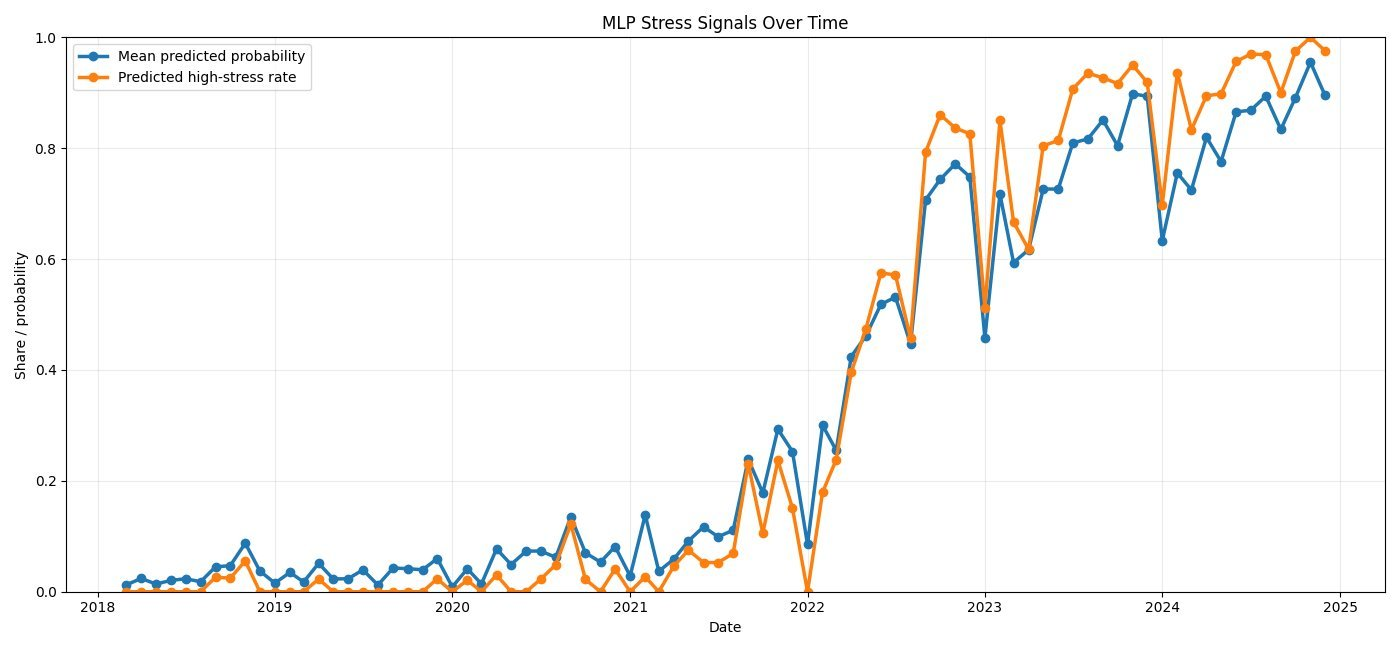
\includegraphics[width=0.99\linewidth]{mlp_stress_trend_over_time.png}
\end{tikzfigure}

\vspace{0.2em}
Both signals hover near zero through 2020, rise in 2021, and climb sharply
through 2022\,--\,2023. By late 2024 the model flagged
\textbf{$\sim$90\% of ZIP codes} as high stress, including historically
accessible neighborhoods like \textbf{Mattapan, Dorchester, and Roxbury Crossing}
that lower and middle income residents have traditionally relied on.

\vspace{0.5em}
\begin{minipage}[t]{0.44\linewidth}
  \centering
  {\large\textbf{Confusion Matrix}}

  \vspace{0.6em}
  {\large
  \begin{tabular}{r|>{\centering\arraybackslash}p{2.4cm}>{\centering\arraybackslash}p{2.4cm}}
    \toprule
    & \textbf{Pred.\ Low} & \textbf{Pred.\ High} \\
    \midrule
    \textbf{True Low}  & 2{,}092 & 378 \\
    \textbf{True High} & 82    & 786 \\
    \bottomrule
  \end{tabular}
  }
\end{minipage}%
\hfill
\begin{minipage}[t]{0.50\linewidth}
  \centering
  {\large\textbf{Classification Metrics}}

  \vspace{0.6em}
  {\Large
  \begin{tabular}{ll}
    Accuracy  & \textbf{86.2\%} \\
    Precision & \textbf{0.68} \\
    Recall    & \textbf{0.91} \\
    F1        & \textbf{0.77} \\
  \end{tabular}
  }
\end{minipage}
}

% =============================================================
%  COLUMN 3 — Key Finding + Bayesian + Conclusions
% =============================================================
\column{0.33}

{
\useblockstyle{AccentBorder}
\block{Key Finding}{
\begin{center}
\vspace{0.1em}
{\fontsize{44}{52}\selectfont\bfseries\color{NEUDarkRed}
Each +1 pp in the mortgage rate\\[4pt]
adds $\sim$\$10{,}000 to the income\\[4pt]
needed to buy a home.}
\end{center}
}
}

\block{{\color{white}\Large 3}\quad Bayesian Regression}{
\begin{tikzfigure}[Posterior means with 95\% credible intervals. Mortgage rate dominates all others by an order of magnitude.]
  
\includegraphics[width=0.99\linewidth]{bayesian_coef_intervals.png}
\end{tikzfigure}

\vspace{0.2em}
\begin{center}
  {\large
  \begin{tabular}{ll}
    \toprule
    Test MAE  & \textbf{\$4{,}306} \\
    Test RMSE & \textbf{\$4{,}481} \\
    Test MAPE & \textbf{2.35\%}  \\
    \bottomrule
  \end{tabular}
  }
\end{center}
}

\block{Conclusions \& Future Work}{
The affordability crisis is no longer confined to expensive neighborhoods like
Back Bay or Cambridge. It has spread into areas that lower and middle income
residents have historically relied on. By late 2024 the MLP classifier flagged
nearly \textbf{90\% of ZIP codes} as high stress. The Bayesian model pinpoints
the mechanism: each percentage point on the mortgage rate translates to roughly
\textbf{\$10{,}000 more income} required to buy a home, with high posterior
certainty. The SARIMAX forecasts confirm the shift was large enough to challenge
even well-specified time series models, particularly in high-value markets
that experienced sharp post-2022 corrections.

\vspace{0.6em}
A return to lower mortgage rates would be the single most impactful lever for
easing stress, but without increased housing supply the underlying price
pressure will persist.

\vspace{0.6em}
\textbf{Limitations.} All three models predict \emph{market-level} pressure
but cannot identify which households within a ZIP code are at risk or have
already been displaced. The income-needed variable is metro-level, flattening
real variation across neighborhoods.

\vspace{0.6em}
\textbf{Future work.} Incorporate ZIP-level demographic and income data to
predict whether current residents can \emph{afford to stay}, not just whether a
neighborhood is expensive. Test Bayesian model robustness on a pre-2018 window
to confirm that the mortgage rate dominance is not specific to the post-pandemic
period.
}

\end{columns}
\end{document}
